\section{Introduction}
\label{sec:int}
%\textbf{Whats the problem?}
Technology is ever advancing and computer systems of today are more powerfull and energy effecient than ever before. These improvments have to a large part the continuos decrease in integrated circuit feature size to thank but as we now are getting close to the physiological limit on how small transistors can become possible improvments have to be looked for elsewhere. The fact that battery powered mobile systems are getting more and more common and that power consupmtion correspons to a large part of the cost in driving the data centers of today makes energy consumption an increasingly big system design constraint.
%\textbf{Why is it important?}

DRAM is the most commonly used memory technique as main memory in computer systems today and represents a groving portion of system power consumption \cite{exascale}. This portion will continue to increase if nothing is done about it and a large part of the DRAM power consumption comes from refreshing all memory-cells in the DRAM. This refreshing has to be done as DRAM store data as a charge in a capacitor and given todays silicon, this charge leak over time. To increase DRAM performance and lower access latencies 3D stacked DRAM has been proposed in which the working temperature will be higher than in regular DRAM. This poses a problem as the rate at which the charge leaks increases with temperature and the DRAM will have to be refreshed more often.   

Power consumption in DRAM consists of two parts, static power and dynamic power. The static power is caused by leakage and the dynamic power is the result of all accesse to the memory. As a refresh basically is the same as a regular read access execpt that the data is not used, and thereby consumes the same amount of energy as a usefull access. As such, a straightforward way to mitigate dynamic DRAM power consumption is to try and reduce the amount of refreshes made. Several different approches on how this can be done exists and some of them will be presented in this paper. Another way to increase power efficency is to do smart scheduling of all DRAM accesses which will give higher performance for the same power consumption. However, this will not be examined in any deeper detail in this paper.  

\begin{figure*}[t]
    \centering
    \subfigure[DRAM throughput loss]{
        \centering
        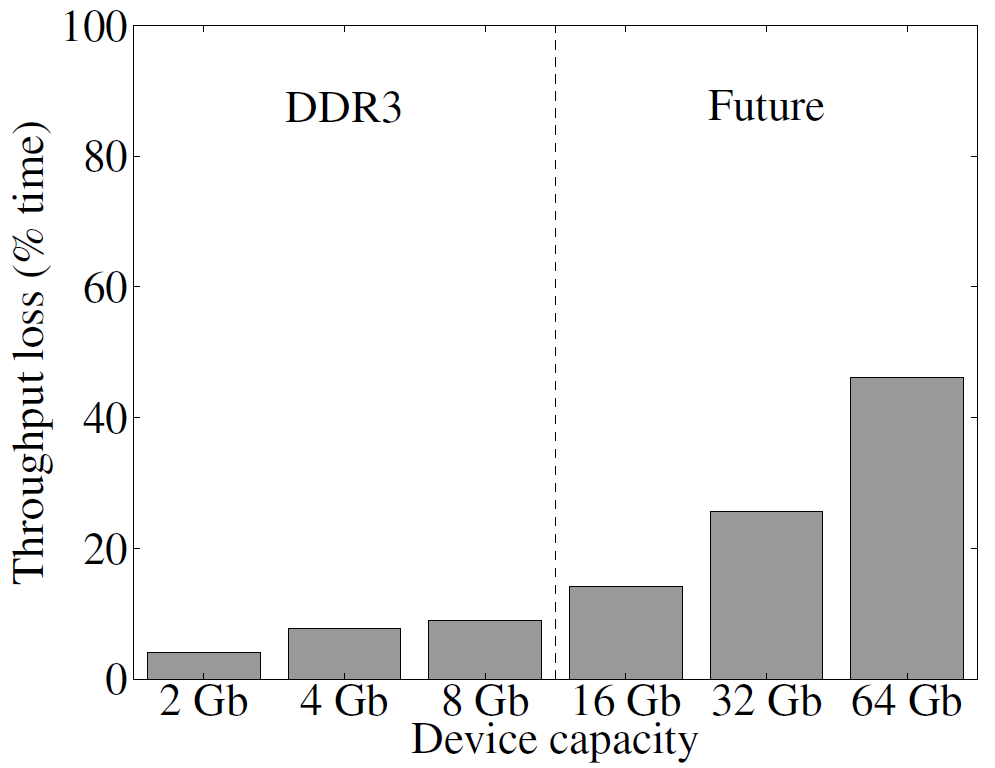
\includegraphics[width=0.45\textwidth]{dram_throughput}
		\label{fig:dram_throughput}
    }
    \subfigure[DRAM power consumption]{
        \centering
        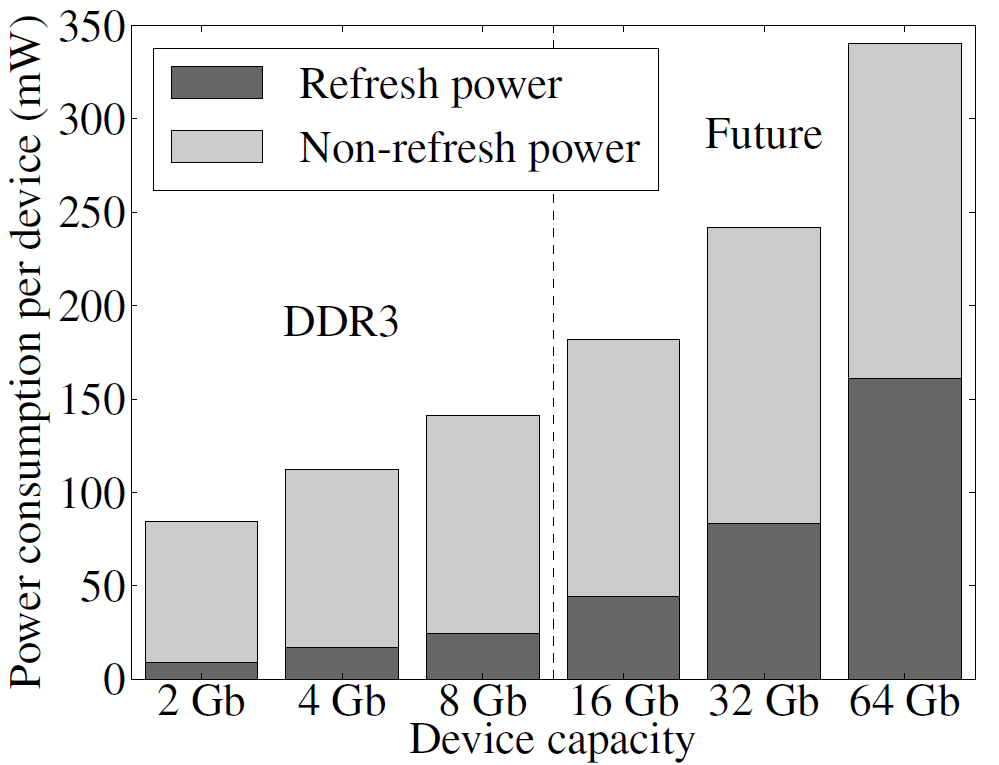
\includegraphics[width=0.45\textwidth]{dram_power}
		\label{fig:dram_power}
    }%
	\caption{Projections on DRAM throughput loss and power consumption \cite{raidr}.}
	\label{fig:dram_data_proj}
\end{figure*}